\chapter{Stars and Supernovae}



\section{Supernovae}


\subsection{Types of supernovae\footnote{Text for Sec. \ref{SNTypes} and Fig. \ref{fig:supernova} are taken from 
 \href{https://astronomy.com/magazine/2004/08/know-your-supernovae}{here}.}} \label{SNTypes}

\begin{figure}[!h]
    \centering
    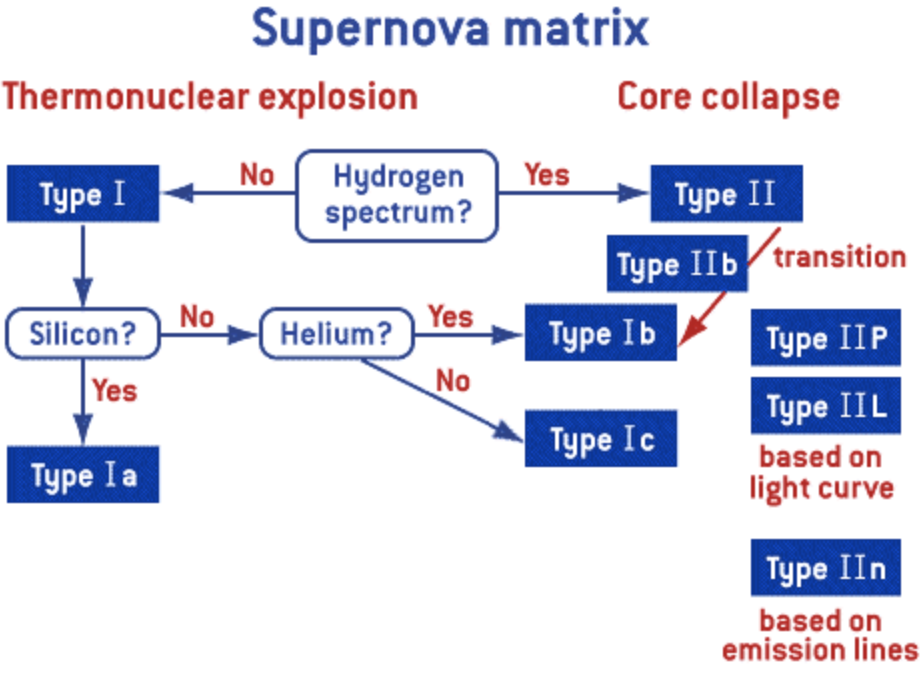
\includegraphics[scale=0.6]{Notes_Images/Supernovae.png}
    \caption{We distinguish supernova types mainly on the basis of their spectra. This illustration relates observed characteristics to the mechanism thought responsible for the explosion.}
    \label{fig:supernova}
\end{figure}

\subsubsection{Type Ia Supernova}

These usually occur in binary systems (two stars orbiting one another) in which one of the stars is a white dwarf. The Type Ia category of supernova produces a fairly consistent peak luminosity because of the fixed critical mass at which a white dwarf will explode - also called Chandrasekar Limit of 1.44 $M_{\odot}$. \textbf{Example}: SN 2001el in NGC 1448

\subsubsection{Types Ib and Ic}

These supernovae types represent the collapse of a massive star. No hydrogen or silicon lines are present in the spectrum, but type Ib spectra show helium. Found only in spiral galaxies, type Ib and Ic supernovae are thought to be associated with massive stars that have lost their hydrogen envelopes either by strong stellar winds (as in Wolf-Rayet stars) or mass loss to a binary companion. Light from these supernovae tends to be more highly polarized, implying more asymmetric explosions among this class. \textbf{Examples: }SN 1998bw (GRB 980425) and SN 2003dh (GRB 030329)

\subsubsection{Type II }

Prominent hydrogen lines are seen in this supernova type's spectrum. These events are associated with regions of recent star formation. They are not found in elliptical or early-type spiral galaxies. This class often is subdivided as IIP (plateau) and IIL (linear) based on how the optical brightness declines. Type IIL supernovae originate from stars retaining much smaller hydrogen envelopes (approximately 1 to 2 solar masses) than progenitors of IIP (typically 10 solar masses) supernovae. \textbf{Example:} SN 1987a in the Large Magellanic Cloud

\subsubsection{Type IIn}

A strong hydrogen spectrum is present with narrow emission lines for this type of supernova. IIn supernovae are thought to originate from the collapse of massive stars embedded in dense shells of material ejected in the decades leading up to the explosion. \textbf{Example}: SN 1998s in NGC 3877

\subsubsection{Type IIb}

The spectrum of this type of supernova contains prominent hydrogen lines right after the event but later transitions to something resembling a Type Ib/c supernova. The progenitor is thought to be a red supergiant that has lost most of its hydrogen envelope either through strong stellar winds or through mass loss to a nearby companion star. IIb supernovae are seen as a "missing link" between supernovae that have retained their envelopes and those that have not. \textbf{Example:} SN 1993j in M81



\section{AGB stars}

Asymptotic Giant Branch (AGB) stars are evolved, low- to intermediate-mass stars ($\sim$ 0.8 − 8M$\odot$) that are characterised by significant mass loss due to a dust-driven wind (Bowen 1988, \href{https://arxiv.org/pdf/2304.05924.pdf}{S. Maes et al. 2023}) As a result, this outflow creates a vast circumstellar envelope (CSE).\\
\\
The type of chemistry in the CSE is set by the elemental carbon-to-oxygen (C/O) ratio of the AGB star, with C/O < 1 resulting in oxygen-rich outflows and C/O > 1 resulting in carbon-rich outflows. AGB outflows with C/O $\sim$ 1 are called \textbf{S-type AGB}. \\
\\
\textbf{Outflow Chemistry:} 
In O-rich AGB outflows, the chemistry is dominated by reactions with the parent species H2O and its daughter OH. Chemistry in C-rich outflows is more diverse since carbon is very reactive, readily producing many carbon-based molecules and ions. 